%%%%%%%%%%%%%%%%%%%%%%%%%%%%%%%%%%%%%%%%%%%%%%%%%%%%%%%%%%%%%%%%%%%%%%%%

%%% LaTeX Template for ECAI Papers 
%%% Prepared by Ulle Endriss (version 1.0 of 2023-12-10)

%%% To be used with the ECAI class file ecai.cls.
%%% You also will need a bibliography file (such as mybibfile.bib).

%%%%%%%%%%%%%%%%%%%%%%%%%%%%%%%%%%%%%%%%%%%%%%%%%%%%%%%%%%%%%%%%%%%%%%%%

%%% Start your document with the \documentclass{} command.
%%% Use the first variant for the camera-ready paper.
%%% Use the second variant for submission (for double-blind reviewing).

\documentclass{ecai} 
%\documentclass[doubleblind]{ecai} 

%%%%%%%%%%%%%%%%%%%%%%%%%%%%%%%%%%%%%%%%%%%%%%%%%%%%%%%%%%%%%%%%%%%%%%%%

%%% Load any packages you require here. 

\usepackage{latexsym}
\usepackage{amssymb}
\usepackage{amsmath}
\usepackage{amsthm}
\usepackage{booktabs}
\usepackage{enumitem}
\usepackage{graphicx}
\usepackage{color}
\usepackage{hyperref}

%%%%%%%%%%%%%%%%%%%%%%%%%%%%%%%%%%%%%%%%%%%%%%%%%%%%%%%%%%%%%%%%%%%%%%%%

%%% Define any theorem-like environments you require here.

\newtheorem{theorem}{Theorem}
\newtheorem{lemma}[theorem]{Lemma}
\newtheorem{corollary}[theorem]{Corollary}
\newtheorem{proposition}[theorem]{Proposition}
\newtheorem{fact}[theorem]{Fact}
\newtheorem{definition}{Definition}

%%%%%%%%%%%%%%%%%%%%%%%%%%%%%%%%%%%%%%%%%%%%%%%%%%%%%%%%%%%%%%%%%%%%%%%%

%%% Define any new commands you require here.

\newcommand{\BibTeX}{B\kern-.05em{\sc i\kern-.025em b}\kern-.08em\TeX}

%%%%%%%%%%%%%%%%%%%%%%%%%%%%%%%%%%%%%%%%%%%%%%%%%%%%%%%%%%%%%%%%%%%%%%%%

\begin{document}

%%%%%%%%%%%%%%%%%%%%%%%%%%%%%%%%%%%%%%%%%%%%%%%%%%%%%%%%%%%%%%%%%%%%%%%%

\begin{frontmatter}

%%% Use this command to specify your submission number.
%%% In doubleblind mode, it will be printed on the first page.

\paperid{363} 

%%% Use this command to specify the title of your paper.

\title{Benchmarking Large Language Models for Bio-Image Analysis Code Generation}

%%% Use this combinations of commands to specify all authors of your 
%%% paper. Use \fnms{} and \snm{} to indicate everyone's first names 
%%% and surname. This will help the publisher with indexing the 
%%% proceedings. Please use a reasonable approximation in case your 
%%% name does not neatly split into "first names" and "surname".
%%% Specifying your ORCID digital identifier is optional. 
%%% Use the \thanks{} command to indicate one or more corresponding 
%%% authors and their email address(es). If so desired, you can specify
%%% author contributions using the \footnote{} command.

\author[A,B]{\fnms{Robert}~\snm{Haase}\orcid{0000-0001-5949-2327}\thanks{Corresponding Author. Email: robert.haase@uni-leipzig.de}}
\author[C]{\fnms{Christian}~\snm{Tischer}\orcid{0000-0003-4105-1990}}
\author[D,B]{\fnms{Nico}~\snm{Scherf}} 

\address[A]{Data Science Center, Leipzig University, Humboldtstra{\ss}e 25, 04105 Leipzig, Germany}
\address[B]{Center for Scalable Data Analytics and Artificial Intelligence (ScaDS.AI) Dresden / Leipzig}
\address[C]{Data Science Centre, European Molecular Biology Laboratory, Meyerhofstra{\ss}e 1, 69117 Heidelberg, Germany}
\address[D]{Max Planck Institute for Human Cognitive and Brain Sciences, Stephanstra{\ss}e 1A, 04103, Leipzig, Germany}

%%% Use this environment to include an abstract of your paper.

\begin{abstract}
In the computational age, life-scientists often solve scientific bio-image analysis (BIA) questions using Python code, even though many of them are not trained in programming. As a common use-case for Large Language Models (LLMs) is code-generation, we see potential in using LLMs for BIA. We present a quantitative benchmark to estimate the capability of LLMs to generate code for solving common BIA tasks. Our benchmark consists of 57 human-written prompts, corresponding reference solutions, written in Python, and unit-tests to evaluate functional correctness of potential solutions. We demonstrate the benchmark by comparing 6 LLMs. We propose mid-/long-term efforts in maintaining and extending the benchmark by the BIA open-source community to ensure community needs are covered properly. This way we can support users when deciding for an LLM and also guide LLM developers in moving the frontier of current capabilities of LLMs towards more advanced applications in BIA. 
\end{abstract}

\end{frontmatter}

%%%%%%%%%%%%%%%%%%%%%%%%%%%%%%%%%%%%%%%%%%%%%%%%%%%%%%%%%%%%%%%%%%%%%%%%

\section{Introduction}

Many projects in biology involve state-of-the-art microscopy and  quantitative bio-image analysis (BIA), which often requires programming skills. As programming is commonly not taught to life-scientists, we see potential in using large language models for this task. Since modern Large Language Models (LLMs) such as chatGPT (OpenAI et al. 2023) were introduced, they change how humans interact with computers. LLMs were originally developed to solve  natural language processing tasks such as  text classification, language translation, or question answering. Interestingly, these models  are also capable of translating human languages, such as English, into programming languages, such as Python. Moreover, they can produce executable code that solves tasks defined by human natural language input \citep{brown2020language}. This capability has huge potential for interdisciplinary research areas such as microscopy bio-image analysis \citep{Royer2023}. LLMs can fill a gap where scientists with limited programming skills meet image analysis tasks which often require knowledge of programming languages. LLMs are indeed capable of writing BIA code as demonstrated in \citep{royer2023omega}, but it is yet unclear where the limitations of this technology are in the BIA context. Multiple LLM code generation benchmarks have been proposed \citep{chen2021evaluating,austin2021,lai2022ds1000,yadav2024pythonsaga,hendrycks2021measuring}. Thus, we think the bioimaging community urgently needs an openly accessible, quantitative way to measure those capabilities in particular given that LLM technology is also developing rapidly. We present such a benchmark, based on HumanEval \citep{chen2021evaluating}, an established code-generation benchmark but ours is tailored for scientific questions in the Bio-Image Analysis context.

\begin{blind}
All code used for the benchmark, sampled prompt-responses from the evaluated LLMs, and Python Jupyter notebooks for reproducing Figures in this preprint are available via this Github repository:
   \url{https://github.com/haesleinhuepf/human-eval-bia}
\end{blind}

%%%%%%%%%%%%%%%%%%%%%%%%%%%%%%%%%%%%%%%%%%%%%%%%%%%%%%%%%%%%%%%%%%%%%%%%

\section{Methods}

Our proposed benchmark consists of 55 human-written Python functions which contain documentation about what the function is supposed to do. An example is shown in Figure 1. We kept the documentation intentionally short, because we intend to use LLMs to facilitate coding for bio-image analysts. This short documentation, the docstring, together with the function signature is passed to an LLM as part of a prompt asking to complete the code. The human-written implementation function body is not passed to the LLM, and just serves as a reference  solution. Additionally, our benchmark provides unit-tests for these python functions to evaluate their functional correctness. If the code generated by  the language model is executable and produces results which pass the unit-tests, this LLM is considered to be able to solve the problem described in the documentation of our function. Every prompt is sent multiple times to the LLM and we measure how often the generated  code passes the tests. Here, we follow the established standard pass@k \citep{chen2021evaluating}, which estimates the probability that, if asked k times, the LLM will at least once give the correct answer. We particularly focus on the practically most relevant special case pass@1 , i.e. we want to know how likely it is that the first generated solution works.  
Our selected prompts range from basic image analysis tasks, such as applying an edge-preserving denoising filter to an image, over intermediate tasks such as labeling objects in a binary image and counting them, shown in Figure \ref{fig:exampletestcase}, to challenging workflows including image processing steps, descriptive statistics, tabular data wrangling and dimensionality reduction. There is also a positive-control test-case, called return\_hello\_world, which is intentionally kept very simple to test if a specific LLM model is  capable of solving a trivial base task at all. A list of all test-cases and corresponding docstrings is given in Supplementary List 1.
To enable future extension and reproducing our benchmark, we provide the necessary infrastructure to turn the list of test-case Jupyter Notebooks into a JSONL file that has the same format as the evaluation framework of HumanEval \citep{chen2021evaluating}. We also did minor modifications to this framework to be able to execute the benchmark for our purposes. For example, we added code that moves example images to a temporary folder from which the test-case code is executed. That way our benchmark can contain operations accessing files and folders, which the original HumanEval benchmark was not capable of. All modifications are explained in our Github repository and the supplementary Zip file. 
We demonstrate the benchmark by comparing the capabilities of a range of state-of-the-art LLMs covering commercial and freely available or open source models: gpt-3.5-turbo-1106, gpt-4-1106-preview, gpt-4-2024-04-09, codellama \citep{roziere2024code}, claude-3-opus-20240229 \citep{anthropic2024claude}, gemini-pro \citep{geminiteam2024gemini}. Code for benchmarking gemini-1.5-pro and gemini-ultra are available as well, but could not be executed due to rate limits. Code for benchmarking Mistral-7B-Instruct-v0.2 \citep{jiang2023mistral} via the Blablador infrastructure of Helmholtz AI is also available. This model was not benchmarked due to technical difficulties at the service provider at the time of benchmarking.
For benchmarking the models, we generated 10 code samples of the 47 test-cases of the 6 models. Benchmarking was done on a Windows 10 Laptop with an AMD Ryzen 9 6900 CPU, 32 GB of RAM and a NVidia RTX 3050 TI GPU with 4 GB of RAM. Codellama, the only locally executed model in our selection, was accessed via ollama version 0.1.29 \citep{ollama2024windows}. The gemini-pro model was accessed via the Google Vertex API \citep{google2024vertex}, which did not support specifying a version. Thus, we document here that the benchmark was executed on April 16th and 17th 2024. 
We also summarize used libraries in the generated code and resulting error messages by counting libraries names and common error messages observed in the results of the code evaluation step.
All test-cases as human-readable Jupyter Notebooks and packaged as JSONL file, sampling and evaluation code, generated samples and data analysis/visualization notebooks are available open-source in the github repository of the project. All respective Python package versions are documented in the environment.yml file in the Github repository and the supplementarty material facilitating full reproducibility of our analysis.

\begin{figure}[h]
\centering
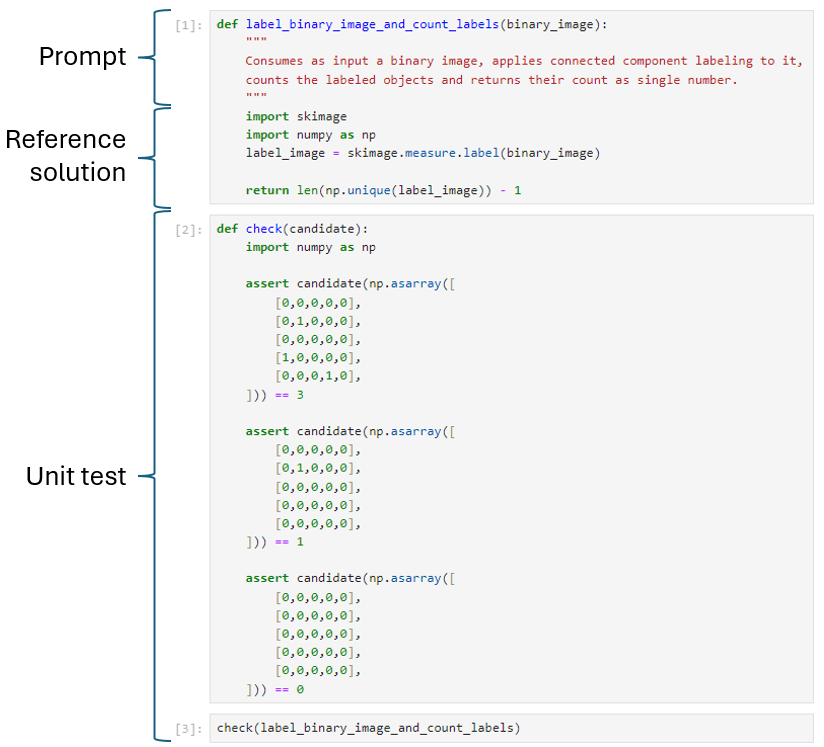
\includegraphics[width=8.5cm]{example_test_case.png}
\caption{The example test-case label\_binary\_image\_and\_count\_labels is implemented as Jupyter Notebook consisting of a function signature consuming a binary image and a docstring describing what the function is supposed to do. These two serve as part of a prompt to the LLM asking to complete the code. The function body serves as a reference solution (sometimes referred to as canonical solution), which allows writing a unit test. If the unit test passes for the code generated by an LLM, indicating functional correctness, the LLM is defined as capable of solving the prompted task. An updated list of all test-cases is available online: 
\url{https://github.com/haesleinhuepf/human-eval-bia/blob/main/test_cases/readme.md}
\newline
\newline
}
\label{fig:exampletestcase}
\end{figure}


%%%%%%%%%%%%%%%%%%%%%%%%%%%%%%%%%%%%%%%%%%%%%%%%%%%%%%%%%%%%%%%%%%%%%%%%

\section{Results}

TODO
Sampling the LLMs using our prompts took approximately 18 hours in total. The models gpt-3.5-turbo-1106, gpt-4-1106-preview, gpt-4-2024-04-09 and claude-3-opus-20240229 caused costs of \$0.23, \$5.10, TODO and \$20.49, respectively. All other models did not cause direct costs as their API usage was free. Comparing the pass rates visualized in Figure \ref{fig:passratellms} reveals that the leading model, gpt-4-1106-preview, managed to answer 42\% of the prompts with code that passed the unit tests. It is followed by claude-4-opus-20240229 and TODO, with 40\% and 28\%, respectively. These numbers correspond to pass@1 counting the success rate from drawn examples. Detailed pass@k rates with k=1, k=5 and k=10 are shown in Supplementary Figure 1. TODO

Detailed pass rate analysis of the individual test-cases, shown in Figure \ref{fig:fig:performancepertask}, highlights that most of the test-cases were solvable by at least one LLM. The positive control, return\_hello\_world, was solved successfully in almost all cases, expressed with a pass-rate of 1.0. Only the codellama model failed in 30\% of the test runs for this particular test-case. Details about which LLM used which Python libraries how often are given in Figure \ref{fig:usedpythonlibs}. Common error messages and corresponding counts how often these were observed when evaluating the generated code are given in Table  TODO.


\begin{figure}[h]
\centering
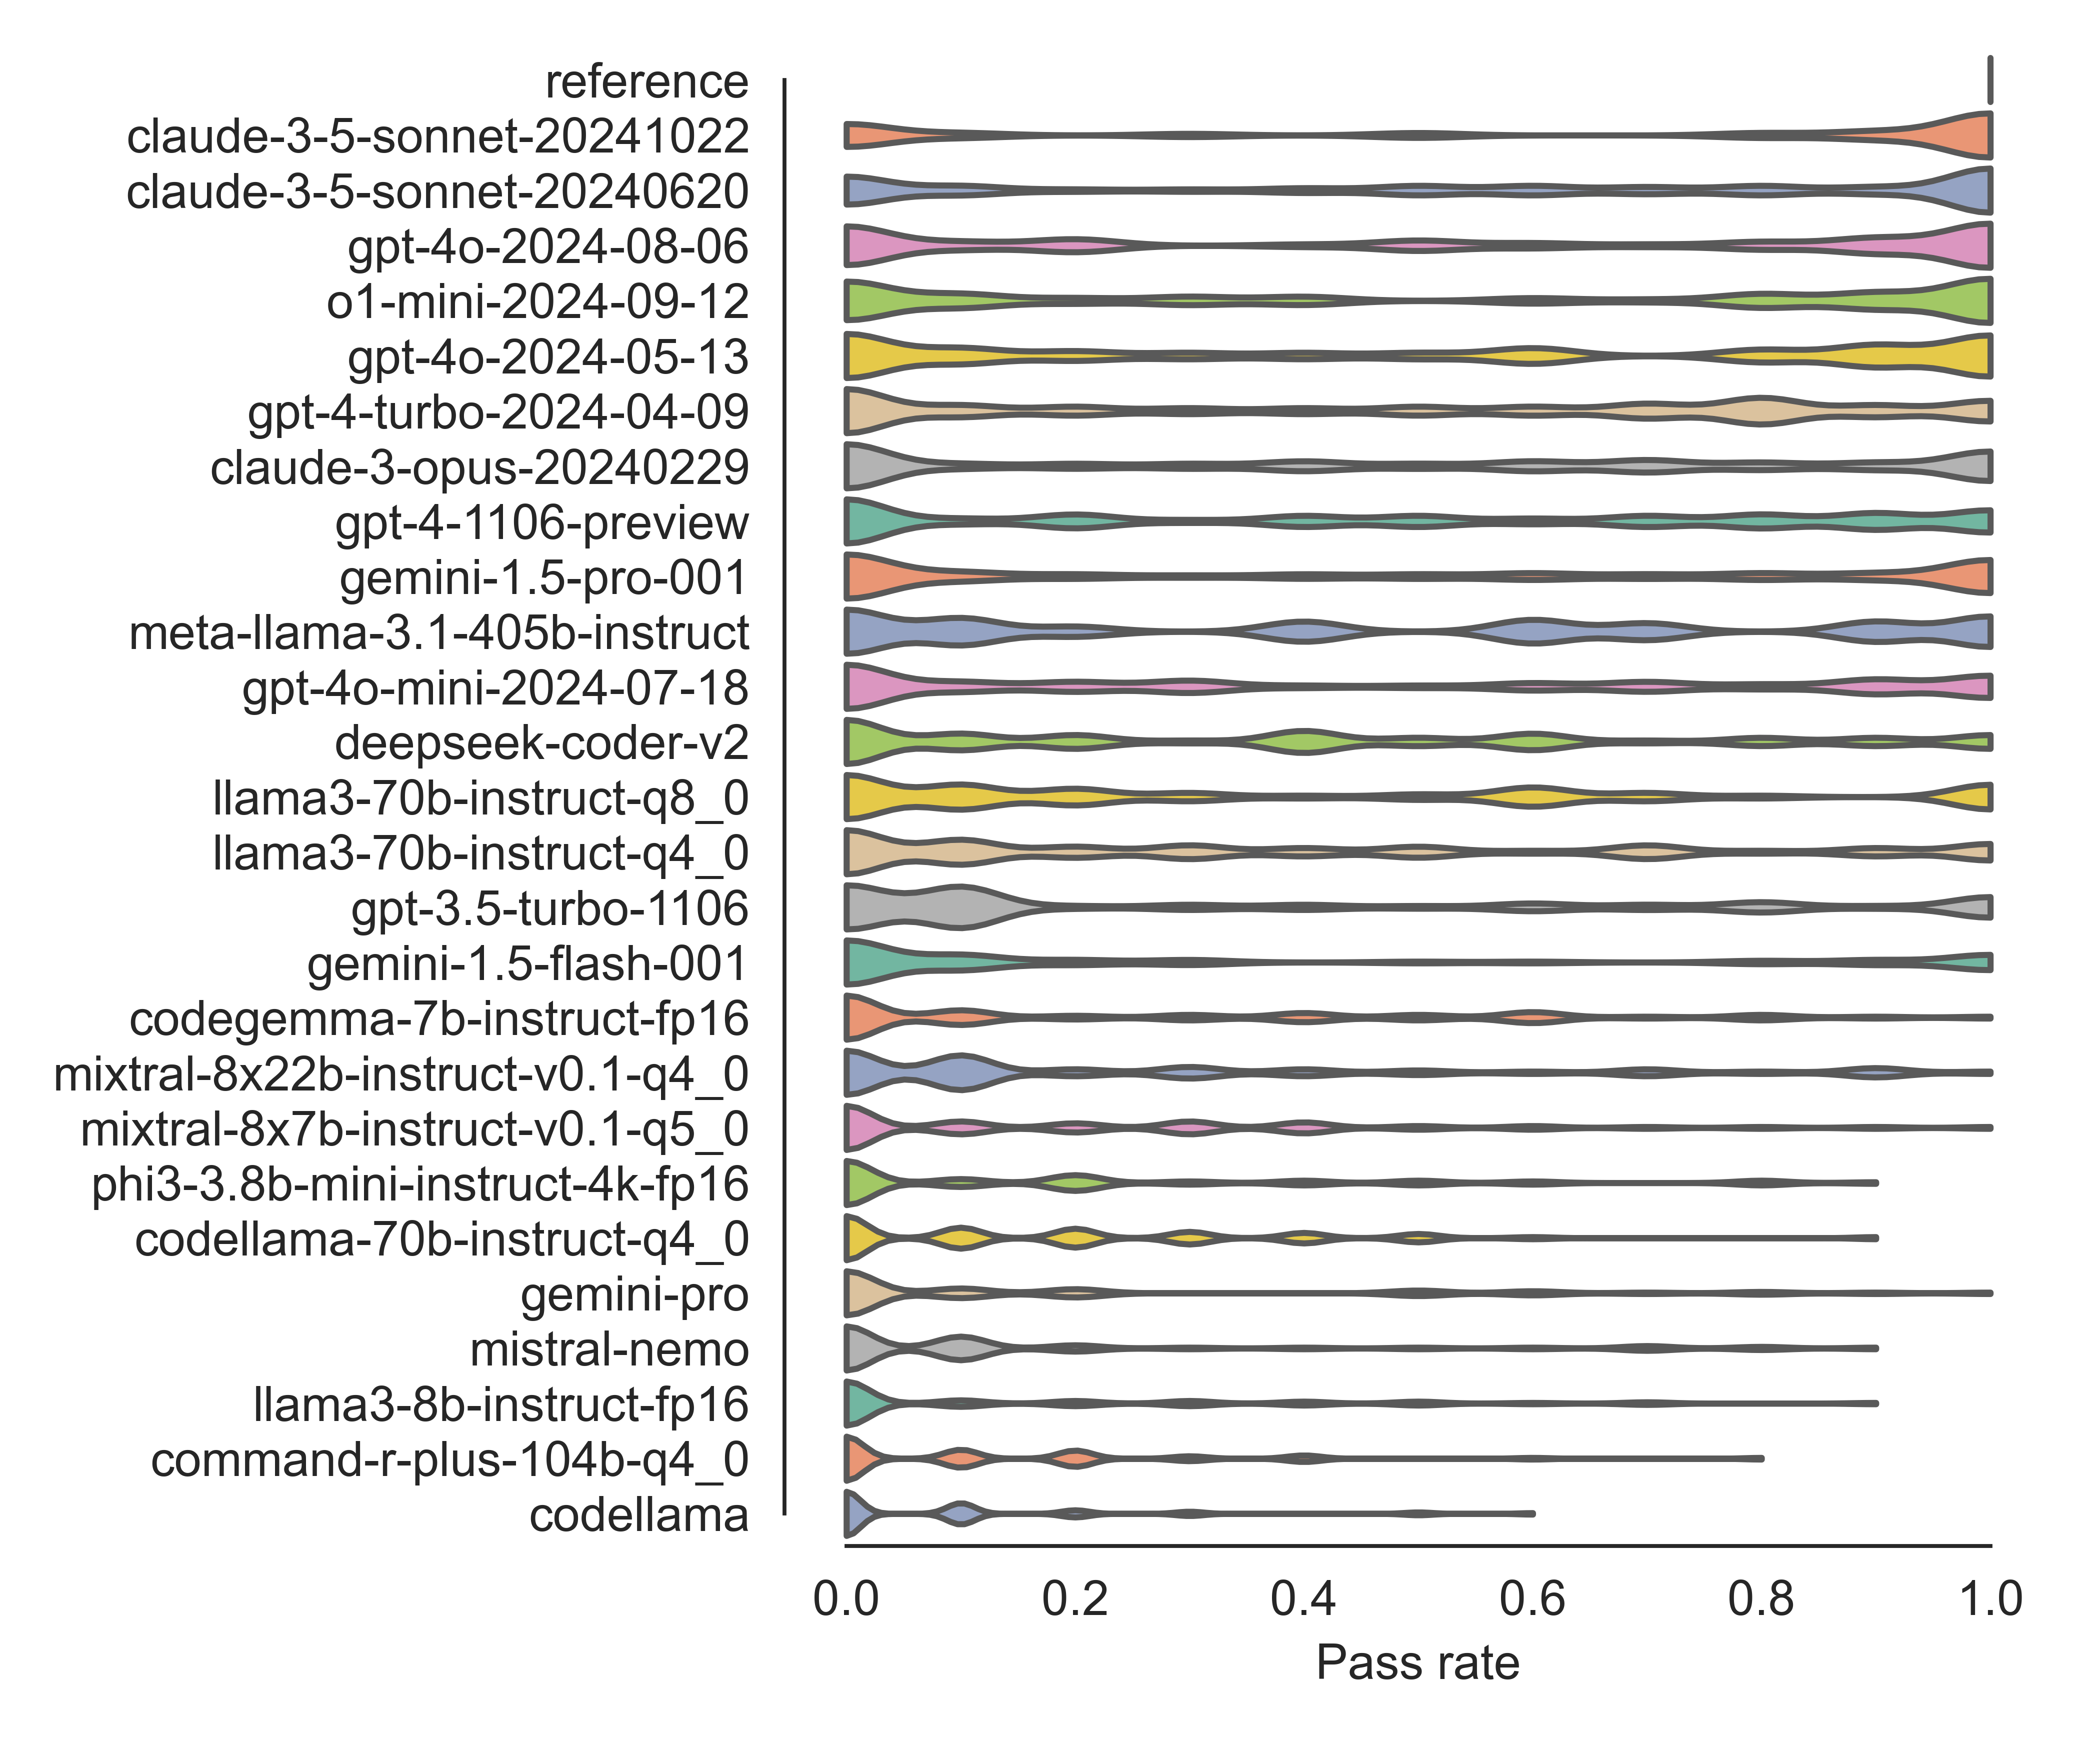
\includegraphics[width=8.5cm]{pass_rate_llms.png}
\caption{Quantitative pass rate comparison of all tested LLMs and, as a sanity check, the human reference solution: Measured fraction of passed tests visualized as box plot summarizing measurements from 47 test-cases. The corresponding, updated notebook is available online: 
\url{https://github.com/haesleinhuepf/human-eval-bia/blob/main/demo/summarize_by_case.ipynb}
\newline
\newline
}
\label{fig:passratellms}
\end{figure}

\begin{figure*}[h]
\centering
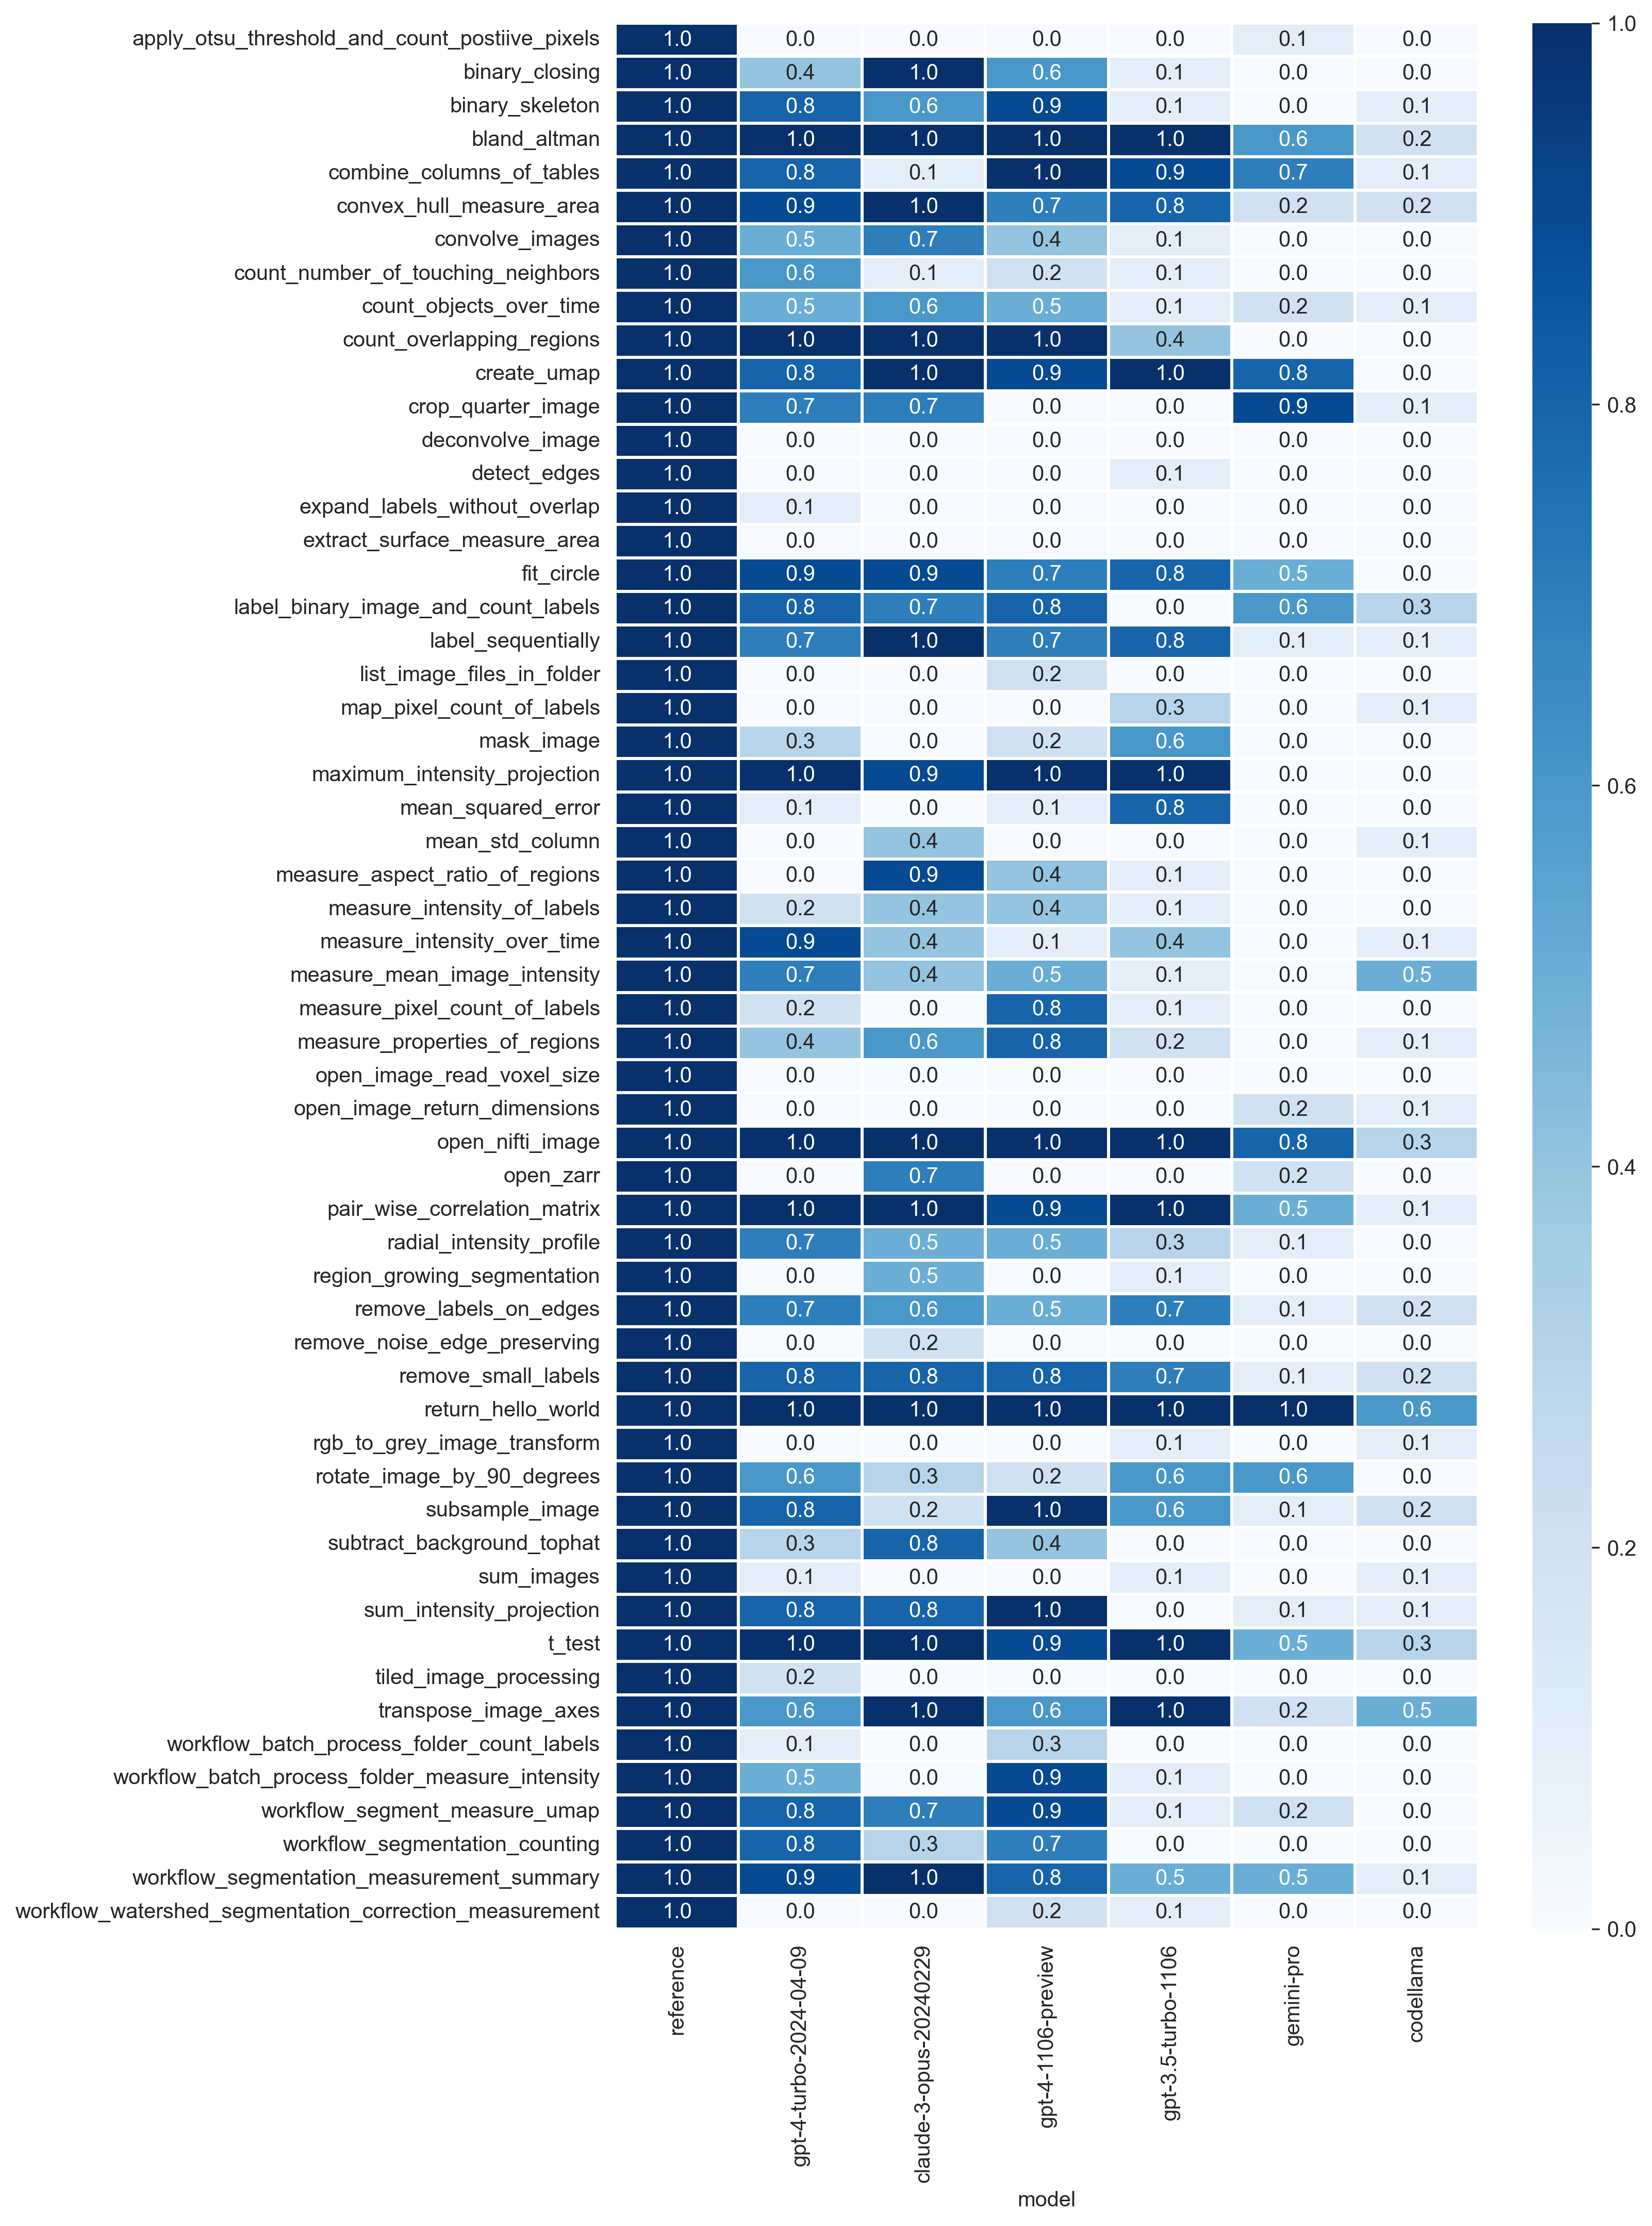
\includegraphics[width=\textwidth]{performance_per_task.png}
\caption{Test-cases  and corresponding pass@1 for each LLM. Pass@1 reports the probability that a generated solution works if a user asks the LLM just a single time. The corresponding, updated notebook is available online:
\url{https://github.com/haesleinhuepf/human-eval-bia/blob/main/demo/summarize_by_case.ipynb}
\newline
\newline
}
\label{fig:performancepertask}
\end{figure*}

\begin{figure*}[h]
\centering
\includegraphics[width=\textwidth]{used_python_libs.png}
\caption{TODO
\url{TODOhttps://github.com/haesleinhuepf/human-eval-bia/blob/main/demo/summarize_by_case.ipynb}
\newline
\newline
}
\label{fig:usedpythonlibs}
\end{figure*}

%TODO:
% 
%Table 1: Snippets of common error messages and how often these were observed when evaluating the generated code. See %https://github.com/haesleinhuepf/human-eval-bia/blob/3e666cf3f3594c255e10a96b68fda58e549d2e26/demo/summarize_error_messages.ipynb 



%%%%%%%%%%%%%%%%%%%%%%%%%%%%%%%%%%%%%%%%%%%%%%%%%%%%%%%%%%%%%%%%%%%%%%%%

\section{Discussion}

We presented a benchmark for comparing code generation capabilities of LLMs in the Bio-Image Analysis context. Such benchmarks are crucial to decide , e.g. if and how to apply this technology in routine projects, training or advanced applications. 
It shall be mentioned that we did not use any code-completion tools, such as github co-pilot, to write the test-cases. It is necessary to not use such LLM-based tools while writing the test-cases, because otherwise we might introduce a bias towards underlying LLMs. For example, github-copilot is based on chatGPT. If the test-cases were written using it, the benchmark might misleadingly reveal better performance of chatGPT.
Inspecting the detailed reports for which test-cases were not solved by any LLM also revealed a couple of cases, which are considered simple, but still were not solvable. Examples are list\_files\_in\_folder, open\_image\_return\_dimensions and rgb\_to\_grey\_transform. Modifying such test-cases now, after a first benchmark has been executed, must be done carefully. A peer-review scheme, e.g. using github pull-requests, is recommended to make sure good scientific practice is maintained. Additionally, we provide tools that enable to detect if the LLMs are attempting to use Python libraries which are not installed yet. These can be added and the evaluation step can be repeated. As we encourage to only add test-cases that can be implemented with common Python libraries, the manual effort for this quality assurance step is limited. When maintaining this benchmark mid-/long-term modifications should be done with care, to not give advantages to specific LLMs.
We limited sample generation for the benchmarking to 10 samples per LLM per test-case. pass@k analysis was done using k=1, k=5 and k=10. The established standard set by \citep{chen2021evaluating} is 200 samples and k=1, k=10 and k=100. As our benchmark is in early development (you are reading a preprint), we considered drawing 200 samples as not well-invested compute time and unnecessary costs. Once the benchmark contains more test-cases and models, this decision may be revised. 
The measured costs also demonstrate the potential of the technology. Requested code is commonly served within seconds, and drawing 300 samples from the 3 paid-per-prompt models causes minimal costs depending on the used model. When using LLMs on a daily basis, it appears unreasonable to draw hundreds of samples. Hence, using LLMs for BIA code generation is affordable and cost-efficient.
Our benchmark is a single-shot benchmark presenting the prompt to the LLM with no history of a former conversation. In daily use, one can interact with LLMs using chat-interfaces and iteratively engineer a prompt. Thus, the tested LLMs may be more capable than measured in our experiment, when used in a chat scenario.
The test-case selection may introduce a certain bias of the sub-discipline we work in. We mostly work with fluorescence microscopy imaging data, showing nuclei and membranes. Most test-cases are derived from practical situations we come across often. Mid-/long-term we hope that community contributions to the benchmark’s github repository will allow us to reflect the field more broadly. For example, algorithms processing histological, hyperspectral, or super-resolution imaging data, would be welcome in our test-case collection. On the other hand, we consider test-cases without practical relevance in bio-image analysis should not be part of the benchmark. For example, an algorithm implementing image-reconstruction techniques for computed tomography, or image-classification algorithms for natural images, showing cats and dogs, should not be included even though they might fit technically in an image-processing benchmark. Also intentionally, we included test-case and prompts which we presume are currently not solvable by any LLM. With this, the benchmark could serve to guide LLM developers in this field.
In our selection of tested LLMs we see two groups of models, and one group seems more capable than the other, expressed by twice as high pass rates. There might be multiple reasons for this: 1) The tested open-source models are much smaller than the tested commercial models, e.g. codellama has 7B parameters and the GPT models are about two orders of magnitude larger. Obviously, model size limits LLM capabilities. 2) In Bio-image Analysis, we use some specific Python libraries, such as aicsimageio \citep{aicsimageio}, vedo \citep{musy2024} or pyclesperanto\_prototype \citep{robert_haase_2023_10432619}, which might not be mentioned in the training data of some models. On the other hand, in natural image processing other libraries such as OpenCV \citep{itseez2015opencv} are used more often than in our field, where scikit-image \citep{scikit-image} is more often used for similar purposes. As natural image processing is also a vivid research field, the LLM’s training data may contain more use-cases from that field. Also the DS-1000 benchmark \citep{lai2022ds1000}, focusing on general data-science use-cases, does not cover scikit-image or opencv. Hence, the test-cases in our benchmark may enable the LLM community to train models covering our BIA use-cases and the libraries established in our field better.
We aim at developing this benchmark further, together with the support by the bio-image analysis community, by adding more test-cases. Furthermore, with the development of the models, we also will adapt the benchmark depending on how LLMs develop. For example, currently upcoming vision-models, LLMs that can take images as input, need to be considered for benchmarking too. The benchmark we presented does not have the capability to test vision-models. Another angle of further development could be efficiency of generated code as proposed earlier \citep{du2024mercury}. In particular in the context of processing 3D+t fluorescence microscopy imaging data, accelerated image processing techniques can by key \citep{Haase2020}. 
\begin{blind}
The presented benchmark could also be used to improve system messages systematically, for example in projects such as napari-chatGPT \citep{royer2023omega} and bia-bob \citep{haase2024biaBob}.
\end{blind}

%%%%%%%%%%%%%%%%%%%%%%%%%%%%%%%%%%%%%%%%%%%%%%%%%%%%%%%%%%%%%%%%%%%%%%%%

\section{Conclusion}

We developed a benchmark for measuring LLM performance in generating code for solving bio-image analysis tasks. It can guide end-users to decide which LLM to use and potentially to pay for when developing bio-image analysis scripts and tools. We also consider this benchmark for LLM-developers in our domain as a metric to guide further development. Last but not least: We encourage the community to send pull-requests with new test-cases to the above-mentioned github repository to ensure the benchmark is covering needs in our field widely. This way, we wish to establish a community-driven approach to benchmarking LLMs for BIA. 


%%%%%%%%%%%%%%%%%%%%%%%%%%%%%%%%%%%%%%%%%%%%%%%%%%%%%%%%%%%%%%%%%%%%%%%%

%%% Use this environment to include acknowledgements (optional).
%%% This will be omitted in doubleblind mode.

\begin{ack}
RH acknowledges the financial support by the Federal Ministry of Education and Research of Germany and by Sächsische Staatsministerium für Wissenschaft, Kultur und Tourismus in the programme Center of Excellence for AI-research „Center for Scalable Data Analytics and Artificial Intelligence Dresden/Leipzig“, project identification number: ScaDS.AI.
Helmholtz AI and the Jülich Supercomputing Centre deserve acknowledgement for providing the blablador infrastructure for testing the mistral model.

\end{ack}

%%%%%%%%%%%%%%%%%%%%%%%%%%%%%%%%%%%%%%%%%%%%%%%%%%%%%%%%%%%%%%%%%%%%%%%%

%%% Use this command to include your bibliography file.

\bibliography{mybibfile}

\end{document}
%%%%%%%%%%%%%%%%%%%%%%%%%%%%%%%%%%%%%%%%%%%%%%%%%%%%%%%%%%%%%%%%%%%%%%
